\chapter[Introdução]{Introdução}


A engenharia por trás da música sempre foi um assunto presente e causador de grandes mudanças. Seguindo uma tendência muito forte nos dias atuais, a engenharia modernizou o mundo da música tirando-a de um mundo analógico e introduzindo ao cenário digital, não só o modo como escutamos as músicas passou a ser digital, mas também o modo como se toca os instrumentos. Em 1996, a modelagem digital de amplificadores valvulados ganhou vida com o lançamento de um amplificador produzido pela \textit{Line 6}, uma empresa americana de instrumentos e acessórios para guitarra. Pela primeira vez na história, um amplificador utilizava um software embarcado em um chip \textit{DSP} (chip digital dedicado para processamento de sinais) como principal componente para timbrar o som do amplificador buscando se aproximar do som produzido por amplificadores valvulados \cite{paulwhite_line6_line6_line6_2006}. O \textit{Axsys 212}, mostrado na figura \ref{fig1} como era chamado, foi um amplificador pioneiro que abriu uma gama de estudos e pesquisas na área de processamento de sinais de áudio.
\begin{figure}[!htb]
	\centering
	{
		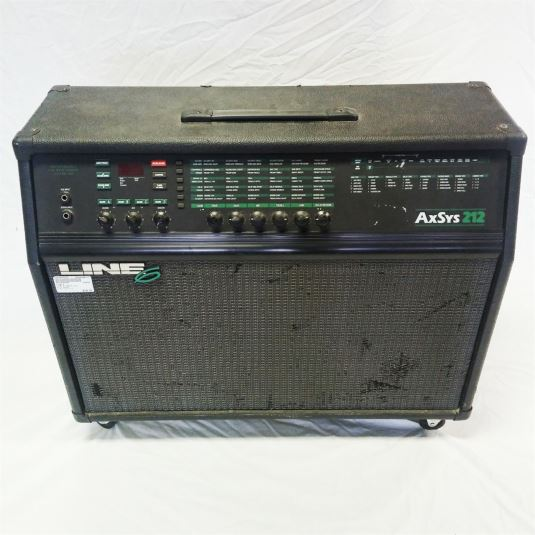
\includegraphics[height=5cm]{figuras/Axsys212}
		\label{Axsys 212}
	}
	\quad %espaco separador
	{
		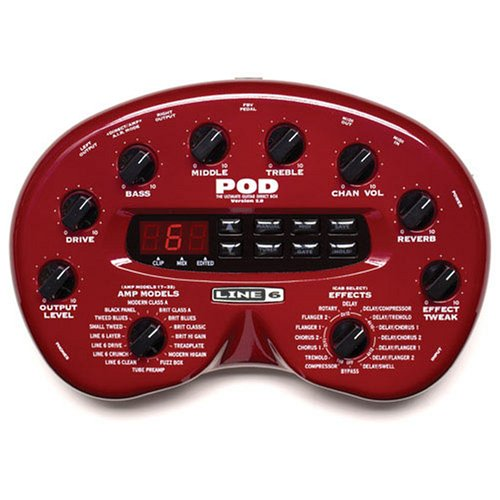
\includegraphics[height=5cm]{figuras/Pod}
		\label{Pod}
	}
	
	\caption{Esquerda: Line 6 Axsys 212. Direita: Line 6 Pod }
	\label{fig1}
\end{figure}




Apesar de toda a inovação, a grande revolução na modelagem de amplificadores começou a ser feita dois anos após o lançamento do \textit{Axsys 212}, com a criação de um simulador portátil de amplificadores, o \textit{POD}, também da \textit{Line 6}, mostrado na figura \ref{fig1}. A qualidade das simulações de amplificadores valvulados na época aumentou consideravelmente e passaram a ser utilizadas para a realização de gravações em estúdios profissionais, onde a qualidade de som é um parâmetro essencial. O uso desses simuladores ganhou grande visibilidade e espaço entre os amplificadores analógicos pelo fato de ser um dispositivo portátil, leve e com uma variedade enorme de timbres, uma vez que um único simulador contém dezenas de modelos de amplificadores diferentes. A modelagem de amplificadores busca extrair todas as características de um amplificador valvulado que personalizam o som que sai da guitarra. 



As válvulas foram muito utilizadas em amplificadores até a invenção dos transistores que tomaram conta da maioria dos amplificadores produzidos atualmente, porém músicos experientes e treinados são capazes de perceber diferenças entre os sons produzidos por amplificadores valvulados e transistorizados. Alguns estudos evidenciam a preferência dos músicos pelos valvulados, onde a diferença predominante para os amplificadores transistorizados é a resposta em frequência de sinais com alta intensidade, ou seja, como amplificador modifica sons graves e agudos \cite{bussey1981tubes}. 

A modelagem desses amplificadores busca caracterizar, com a maior fidelidade possível, o modo como as válvulas tratam sinais de áudio. Como a saturação, ou distorção, gerada pelas válvulas é muito mais suave do que as distorções geradas por transistores, os amplificadores valvulados tendem a ter um som mais agradável ao ouvido humano. 

Os amplificadores valvulados, basicamente, são compostos por:

\tikzstyle{int}=[draw, fill=blue!20, minimum size=2em]
\tikzstyle{init} = [pin edge={to-,thin,black}]
\begin{figure}	[!htb]
	\centering
	
	
	\begin{tikzpicture}[node distance=3cm,auto,>=latex']
	
	\node (a) {Pré};
	\node (b)  {a};
	
	\node [int] (a) {Pré};
	\node [int] (c) [right of=a] {Equalização};
	\node [int] (d) [right of=c] {Power};
	\node (b) [left of=a,node distance=2.5cm, coordinate] {a};
	\node [coordinate] (end) [right of=d, node distance=2.5cm]{};
	\path[->] (b) edge node {Entrada} (a);
	\path[->] (a) edge node {} (c);
	\path[->] (c) edge node {} (d);
	\draw[->] (d) edge node {Saída} (end) ;
	
	
	\end{tikzpicture}
	\caption{Diagrama dos Principais componentes de um amplificador de guitarra}
	\label{Diagrama01}
\end{figure}

\begin{itemize}
	\item Pré: Pré amplificação, é o primeiro estágio de amplificação onde ocorre a primeira saturação, ou seja o primeiro estágio não linear, geralmente composto por válvulas do tipo triodo e um controle de volume;
	\item Equalização: Parte linear encarregada de filtrar o sinal, geralmente é divida em 3 bandas, sendo essas, graves, médios e agudos;
	\item \textit{Power}: Do Inglês, é a Potência, responsável por mais um estágio de amplificação, geralmente composto de pentodos, onde a saturação ocorre devido a uma forte não linearidade presente nas válvulas;
\end{itemize}

A modelagem de cada um dos estágios mostrados na figura \ref{Diagrama01} pode ser separada em duas classes:

\begin{itemize}
	\item Sistemas Lineares: Equalização;
	\item Sistemas Não Lineares: Pré amplificação e Amplificação de potência; 
\end{itemize}


A modelagem de amplificadores pode ser baseada então em algumas categorias como: aproximação por caixa preta (\textit{black box approach}), análise de todos os componentes discretizados (\textit{white box approach}), função de transferência linear e não linear entre muitas outras que podem ser vistas com mais detalhes em \cite{pakarinen2009review}.

Além da modelagem digital é possível também modelar amplificadores de forma analógica. Em 1993 uma empresa chamada Tech 21, lançou um pedal de guitarra (SansAmp GT2) que incorporava as características do som de um amplificador valvulado, como a incorporação de harmônicos e distorções simétricas causadas pelas válvulas. Com uma operação muito simples o SansAmp GT2, mostrado na figura \ref{fig:sansamp}, possui três modelos de amplificadores diferentes, cada um desses amplificadores modelados foram baseados em amplificadores famosos sendo eles: Mesa/Boogie para o California, Marshall para o \textit{British} e Fender para o \textit{Tweed}. Cada um dos amplificadores possui três opções de timbre, com a chave MOD, é possível escolher três modos que modificam a distorção do sinal. Também existe a opção de alterar a emulação da posição do microfone que supostamente estaria captando o som do amplificador. Além dessas opções o pedal conta com um controle de volume, um equalizador de duas bandas e um ajuste de ganho.
\begin{figure}[!htb]
	\centering
	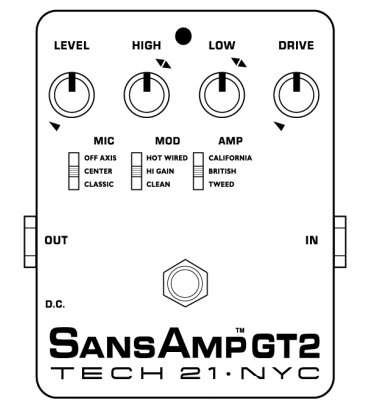
\includegraphics[width=0.7\linewidth]{figuras/SanSamp}
	\caption{SansAmp GT2 .Fonte: Manual do Usuário do SansAmp GT2}
	\label{fig:sansamp}
\end{figure}

Este pedal foi bastante utilizado durante muitos anos, por ser puramente analógico e pela baixa qualidade do som da modelagem digital no seu início. Muitos músicos possuem preconceitos contra a utilização de equipamentos digitais e preferem utilizar apenas equipamentos totalmente analógicos.


\section*{O problema a ser abordado}
Os amplificadores de guitarra sempre foram um dos principais elementos entre todos os equipamentos necessários para um guitarrista. É indispensável para um som de qualidade, um amplificador que possua bons timbres e, na história dos amplificadores existem modelos que ficaram consagrados por timbres únicos e diferenciados. Até pouco tempo atrás, para se reproduzir o som de um amplificador de época - como são chamados os modelos com timbres diferenciados - era necessário possuir o amplificador em questão. O surgimento de técnicas de processamento digital de sinais permitiu reproduzir características desses amplificadores em dispositivos pequenos e portáteis, possibilitando assim, uma grande variedade de modelos de amplificadores famosos sem o problema de ter que se possuir os modelos físicos. Desde a sua criação, a modelagem digital de amplificadores valvulados vem se reinventando desde a sua criação. Sempre inovando na forma com que os amplificadores são modelados e na qualidade do som. O surgimento do \textit{Kemper Profiling Amp}, em 2013, mostrado na figura \ref{fig:profilingampbk-large}, trouxe uma nova visão ao mundo da modelagem de amplificadores. Este dispositivo realiza, em tempo real, a emulação de amplificadores valvulados através do método de caixa preta, ou seja, sem conhecer o circuito do amplificador e nem quais componentes constituem o amplificador.

\begin{figure}[!htb]
	\centering
	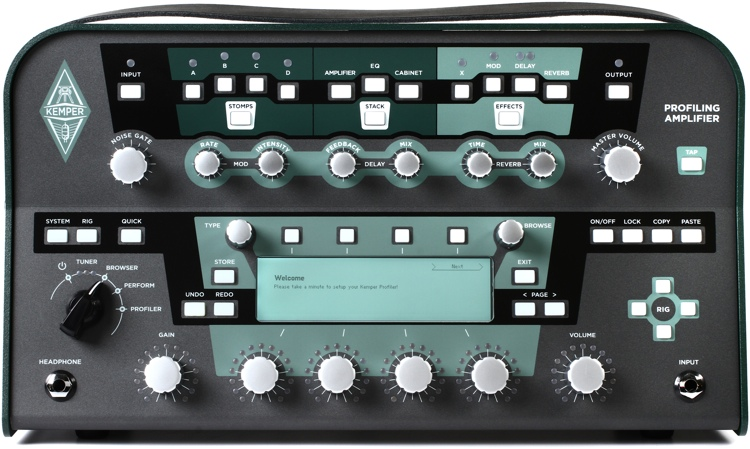
\includegraphics[width=0.7\linewidth]{figuras/ProfilingAmpBK-large}
	\caption{Amplificador Kemper Profiling Amp}
	\label{fig:profilingampbk-large}
\end{figure}




O funcionamento do \textit{Kemper} se dá da seguinte maneira: ele é um amplificador de guitarra capaz de modelar qualquer amplificador, realizando como se fosse uma mímica do timbre produzido por qualquer amplificador. Isso é feito a partir da aplicação de sinais no amplificador que se deseja imitar, ou como o nome do amplificador diz, criar um perfil(\textit{profiling}) e gravar a saída desses sinais, realizado diretamente no dispositivo sem precisar de periféricos de gravação de áudio. Assim, de maneira automatizada, o \textit{Kemper} gera um modelo digital do amplificador físico que foi utilizado e salva em uma memória para que possa ser utilizado futuramente. Esse processo basicamente tira uma fotografia do modo como o amplificador está configurado, adicionando equalizadores e outros efeitos. Além disso, é possível refinar o modelo criado tentando se aproximar ainda mais do som original do amplificador analógico.

A modelagem feita por esse amplificador depende então de se possuir o amplificador de referência para que os sinais possam ser aplicados e o amplificador então pode gerar o modelo digitalizado do amplificador. Para contornar o problema de ter que possuir todos os amplificadores que se deseja modelar, é possível inserir modelos já prontos através do compartilhamento de arquivos via Internet. Uma pessoa que já tenha realizado uma modelagem de um amplificador qualquer, pode disponibilizar para todos os usuários do \textit{Kemper} um arquivo que contém um certo amplificador modelado, com isso é possível inserir vários modelos no amplificador.

O \textit{Kemper}, faz uso de técnicas não paramétricas para modelar os amplificadores. Técnicas não paramétricas são técnicas que modelam apenas como o amplificador modifica o som, ou seja, são técnicas que relacionam o sinal de entrada do amplificador com a saída. Elas não dependem de nenhum componente interno. De forma semelhante este trabalho busca modelar amplificadores de época através de técnicas não paramétricas, como as séries de Volterra.

As séries de Volterra, criada por Vito Volterra em 1930, é uma das primeiras de caracterização sistemática de sistemas não lineares, essencialmente é uma extensão da convolução de sistemas lineares para sistemas não lineares \cite{cheng2017volterra}. Como as válvulas que compõem os amplificadores são dispositivos não lineares, que funcionam através do efeito termoiônico, o modelo de \textit{Hammerstein} da série de Volterra é ideal para realizar a modelagem de um amplificador valvulado






\section*{Objetivos}
\subsection*{Objetivos Gerais}
O método e os sinais utilizados pelo \textit{Kemper} permanecem em segredo da empresa. Além disso as técnicas de modelagem como amplificadores são complexas e dependem de um conhecimento muito específico para serem aplicadas. Técnicas não paramétricas que poderiam ser utilizadas de forma automatizada, extraem os parâmetros lineares dos amplificadores. No entanto, a principal característica que constitui um amplificador valvulado é a forma não linear que o som é distorcido.

O estudo sobre séries de Volterra foi uma das formas encontradas para se analisar e caracterizar sistemas não lineares, como amplificadores valvulados. Essa série permite a realização de uma análise de sistemas não lineares através de coeficientes chamados \kernels da série de Volterra. Esses \kernels são respostas ao impulso do amplificador em análise e, apesar da sua difícil obtenção, podem ser obtidos através de diferentes formas que serão abordadas nos próximos capítulos.

Sabendo que a maior parte dos estudos de modelagem tem foco em 
características lineares dos amplificadores, este trabalho tenta melhorar a modelagem de amplificadores de áudio incluindo 
componentes não-lineares desses amplificadores. Nossa intensão é que essa modelagem se aproxime mais do som real 
dos amplificadores de época.

\subsection*{Objetivos Específicos}
\begin{itemize}
	\item Estudar técnicas de modelagem
	\item Criar vetores de testes para extrair parâmetros lineares e não lineares
	\item Realizar testes em um amplificador valvulado
	\item Comparar os resultados obtidos com os esperados
	\item Criar um modelo do amplificador real usando os parâmetros obtidos
	\item Replicar o som usando apenas o modelo.
\end{itemize}
